\documentclass[11pt,a4paper]{article}
\usepackage[utf8]{inputenc}
\usepackage[T1]{fontenc}
\usepackage{array}
\usepackage{amsmath}
\usepackage{amsfonts}
\usepackage{siunitx}
\usepackage{placeins}
\usepackage{amssymb}
\usepackage{makeidx}
\usepackage{sidecap}
\usepackage{fvextra}
\usepackage{multicol}
\usepackage{listings}
\usepackage{appendix}
\usepackage{comment}
\usepackage{nicematrix}
\usepackage{multirow}
\usepackage{braket}
\usepackage{graphicx}
\usepackage{relsize}
\usepackage{fancyhdr}
\usepackage{cprotect}
\usepackage{color} 
\usepackage{hyperref}
\hypersetup{
	colorlinks=true, 
	linktoc=all, 
	linkcolor=blue,
	urlcolor=blue
}
\usepackage[left=2cm,right=2cm,top=1.5cm,bottom=2cm]{geometry}
\usepackage{titling}
\usepackage{etoolbox}
\flushbottom
\title{Statistical Analysis of Experimental Data\\
	\vspace{0.2cm}
	\large{Homework 06}}
\vspace{-0.2cm}
\author{Igor Di Tota}
\date{\small \url{https://github.com/igordt/SAED_homeworks/tree/main}}


\begin{document}
	
	\maketitle
	
	\section*{Introduction}

	This homework concerns frequentist parameter inference: \textit{consider a sample of 10 measurements from the normal distribution $G(\mu, \sigma)$. Assuming that the measured variance of the sample is $\hat\sigma^2 = \langle x^2 \rangle - \langle x \rangle^2 = 4$, calculate the frequentist 95\% CL upper limit on the true variance of the distribution, $\sigma^2$, based on the properties of the Gamma distribution, and verify the result by the means of the Monte Carlo simulation.}

	The variance of the sample is estimated as
	\begin{equation}
		\hat\sigma^2 = \langle x^2 \rangle - \langle x \rangle^2 = \frac{1}{N}\sum_{i=1}^{N} (x_i - \bar{x})^2 ,
	\end{equation}
	which is the maximum likelihood estimator of $\sigma^2$ when the mean is also estimated from the same data.
	This estimator is biased, since the Bessel correction ($N-1$ instead of $N$) is missing; however, since the frequentist limit is built directly from the probability distribution of $\hat\sigma^2$, the bias is taken into account.

	Following the Neyman construction, the limit is derived from the probability distribution of the measured quantity $\hat\sigma^2$ for a given value of the parameter $\sigma^2$.

	\section*{Distribution of the variance estimator}

	The estimator $\hat\sigma^2$ is itself a random variable.
	As shown in the lecture, the quantity
	\begin{equation}
		z = \frac{N \hat\sigma^2}{\sigma^2} = \sum_{i=1}^{N} \left(\frac{x_i - \bar{x}}{\sigma}\right)^2
	\end{equation}
	is distributed according to the Gamma distribution
	\begin{equation}
		f(z; k, \lambda) = \frac{\lambda^k z^{k-1} e^{-\lambda z}}{\Gamma(k)}, \qquad k = \frac{N-1}{2}, \quad \lambda = \frac{1}{2}.
	\end{equation}
	This particular case of the Gamma distribution is the $\chi^2$ distribution with $N-1$ degrees of freedom: $z$ is a sum of squares of standardized Gaussian variables, with one degree of freedom lost because the mean is estimated from the same data (constraint $\sum_i (x_i - \bar{x}) = 0$).
	
	Some properties of the estimator follow directly:
	\begin{itemize}
		\item the expected value is $\langle \hat\sigma^2 \rangle = \frac{N-1}{N}\sigma^2 = 0.9\,\sigma^2$, so the ML estimator is biased;
		\item the distribution is asymmetric, with the most probable value at $\frac{N-3}{N}\sigma^2 = 0.7\,\sigma^2$;
		\item the probability of measuring a value below the true one is given by the cumulative distribution function of the Gamma distribution, $P(\hat\sigma^2 < \sigma^2) = P(z < N) = F_z(N) = 0.650$.
	\end{itemize}
	Because of this asymmetry, the confidence interval on $\sigma^2$ is not symmetric around the measured value.

	\subsection*{Monte Carlo check of the distribution}

	Before using the Gamma distribution to compute the limit, it is checked with a Monte Carlo simulation.
	$10^6$ experiments are generated, each one consisting of $N = 10$ measurements drawn from $G(\mu, \sigma)$ with $\mu = 0$ and $\sigma^2 = 4$; the value of $\mu$ is irrelevant, since $\hat\sigma^2$ does not depend on it.
	For each experiment the variance is estimated without the Bessel correction (\texttt{np.var} with \texttt{ddof=0}).

	The probability density of $\hat\sigma^2$ for a given true variance is obtained from the one of $z$ with a change of variable.
	Since $z = N\hat\sigma^2/\sigma^2$ is a bijective function of $\hat\sigma^2$, the probability contained in corresponding intervals must be the same:
	\begin{equation}
		f(\hat\sigma^2; \sigma^2)\, d\hat\sigma^2 = f_z(z)\, dz
		\quad\Rightarrow\quad
		f(\hat\sigma^2; \sigma^2) = f_z\big(z(\hat\sigma^2)\big) \left|\frac{dz}{d\hat\sigma^2}\right| = \frac{N}{\sigma^2}\, f_z\!\left(\frac{N \hat\sigma^2}{\sigma^2}\right),
	\end{equation}
	where the factor $N/\sigma^2$ is the Jacobian of the transformation.

	The histogram of the generated values is compared with this density in Figure~\ref{fig:s2_distribution}.
	The mean value and the fraction of results below the true variance also agree with the expected ones:
	\begin{equation}
		\langle \hat\sigma^2 \rangle_{\text{MC}} = 3.5969 \quad (\text{expected } 3.6000), \qquad
		P(\hat\sigma^2 < \sigma^2)_{\text{MC}} = 0.6501 \quad (\text{expected } 0.6495).
	\end{equation}

	\begin{figure}[!h]
		\centering
		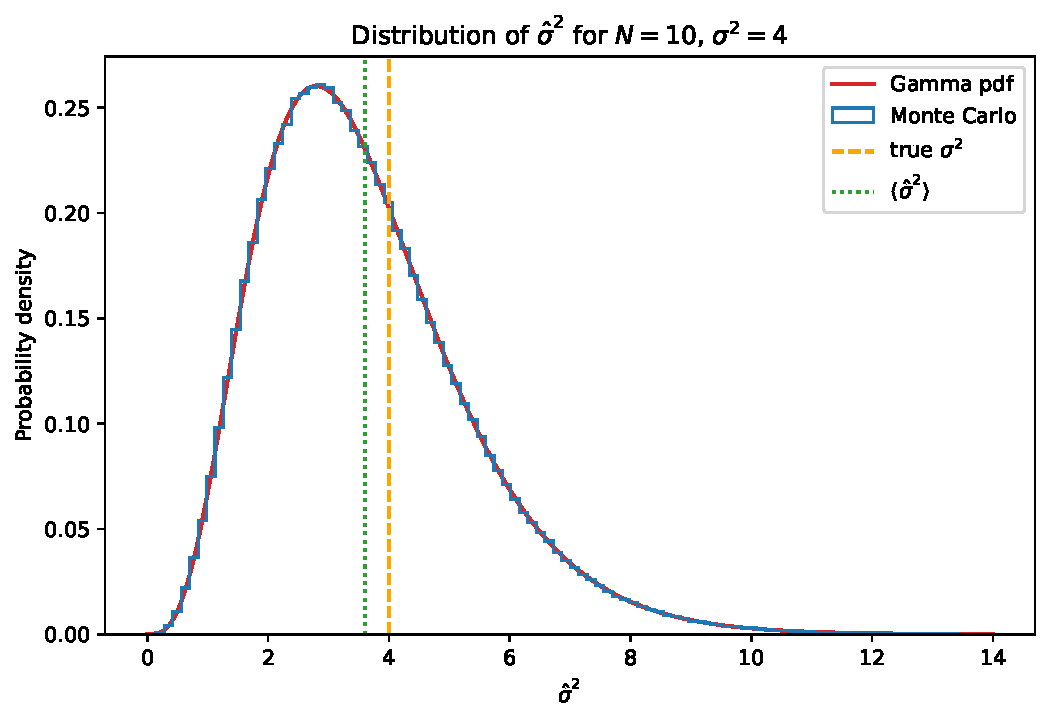
\includegraphics[width=0.6\linewidth]{images/s2_hat_distribution.pdf}
		\caption{Distribution of $\hat\sigma^2$ for $N = 10$ and $\sigma^2 = 4$: Monte Carlo histogram compared with the density obtained from the Gamma distribution. The dashed and dotted lines show the true variance and the expected value $\langle\hat\sigma^2\rangle$.}
		\label{fig:s2_distribution}
	\end{figure}
	\FloatBarrier

	\section*{Analytic upper limit}

	In the frequentist approach, a value of the true variance $\sigma^2$ is excluded if, assuming it is true, a result as small as the measured one, or smaller, would be obtained with a probability lower than $\alpha = 1 - \text{CL}$.
	Small measured values of $\hat\sigma^2$ are unlikely for large values of $\sigma^2$, so this condition defines an upper limit $\sigma^2_{ul}$:
	\begin{equation}
		P(\hat\sigma^2 \leq \hat\sigma^2_m;\ \sigma^2_{ul}) = \alpha = 0.05,
	\end{equation}
	where $\hat\sigma^2_m = 4$ is the measured value.
	The probability is always computed for the random variable $\hat\sigma^2$, for a fixed value of the parameter $\sigma^2$.

	Using $z = N\hat\sigma^2/\sigma^2$, this probability can be written in terms of the cumulative distribution function $F_z$ of the Gamma distribution:
	\begin{equation}
		P(\hat\sigma^2 \leq \hat\sigma^2_m;\ \sigma^2) = P\!\left(z \leq \frac{N\hat\sigma^2_m}{\sigma^2}\right) = F_z\!\left(\frac{N\hat\sigma^2_m}{\sigma^2}\right).
	\end{equation}
	This is a decreasing function of $\sigma^2$, so all values $\sigma^2 > \sigma^2_{ul}$ are excluded at 95\% CL.

	To solve this condition, let $z_\alpha$ be the point where the area under $f_z$ to its left is equal to 5\%:
	\begin{equation}
		F_z(z_\alpha) = \int_0^{z_\alpha} f_z(z)\, dz = \alpha .
	\end{equation}
	The condition for the limit reads $F_z\!\left(N\hat\sigma^2_m/\sigma^2_{ul}\right) = \alpha = F_z(z_\alpha)$.
	Since $F_z$ is strictly increasing, two values with the same cumulative probability must coincide, so
	\begin{equation}
		\frac{N\hat\sigma^2_m}{\sigma^2_{ul}} = z_\alpha
		\quad\Rightarrow\quad
		\sigma^2_{ul} = \frac{N\hat\sigma^2_m}{z_\alpha}.
	\end{equation}
	The value $z_\alpha$ is obtained in SciPy with the method \texttt{ppf} (percent point function), which returns the value of $z$ corresponding to a given cumulative probability.
	The result is
	\begin{equation}
		z_\alpha = 3.3251, \qquad \sigma^2_{ul} = 12.030, \qquad \sigma_{ul} = 3.468 .
	\end{equation}
	The construction is shown in Figure~\ref{fig:ul_analytic}.

	\begin{figure}[!h]
		\centering
		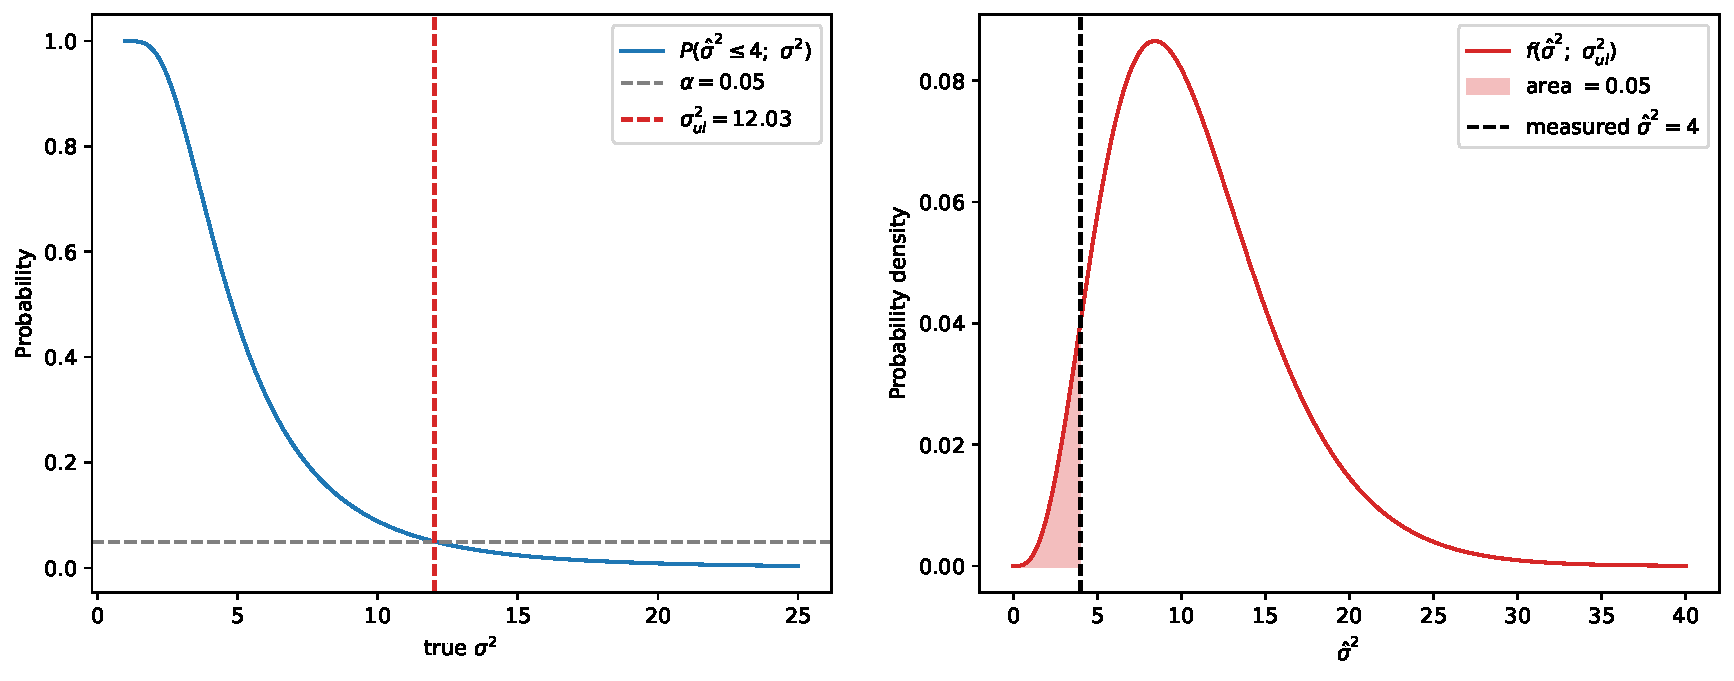
\includegraphics[width=\linewidth]{images/upper_limit_analytic.pdf}
		\caption{Left: probability $P(\hat\sigma^2 \leq 4;\ \sigma^2)$ as a function of the true variance; the upper limit is where it crosses $\alpha = 0.05$. Right: distribution of $\hat\sigma^2$ for $\sigma^2 = \sigma^2_{ul}$; the shaded area below the measured value is equal to $\alpha$.}
		\label{fig:ul_analytic}
	\end{figure}
	\FloatBarrier

	\section*{Monte Carlo verification of the upper limit}

	The upper limit is now obtained again without using the Gamma distribution, by following directly the Neyman construction with simulated experiments.
	For each value of the true variance $\sigma^2$ on a grid of 41 values between 4 and 24, $n = 2 \times 10^5$ pseudo-experiments are generated, each one made of $N = 10$ measurements drawn from $G(0, \sigma)$, and the variance $\hat\sigma^2$ is computed for each of them.

	From the simulated values two quantities are extracted:
	\begin{itemize}
		\item the fraction of experiments with $\hat\sigma^2 \leq \hat\sigma^2_m = 4$, which estimates $P(\hat\sigma^2 \leq \hat\sigma^2_m;\ \sigma^2)$. The upper limit is the value of $\sigma^2$ where this fraction is equal to $\alpha = 0.05$;
		\item the 5\% quantile $\hat\sigma^2_{ll}(\sigma^2)$ of the simulated values, which is used to draw the confidence belt. For each $\sigma^2$, the horizontal segment $\hat\sigma^2 \geq \hat\sigma^2_{ll}(\sigma^2)$ contains 95\% of the possible measurements. Together, the segments form the accepted region, bounded on the left by the curve $\hat\sigma^2_{ll}(\sigma^2)$. The measurement $\hat\sigma^2_m = 4$ is a vertical line. The upper limit is the value of $\sigma^2$ where this line meets the boundary of the accepted region.
	\end{itemize}

	The fraction estimated from $n$ experiments has a binomial uncertainty $\sqrt{p(1-p)/n}$.
	The value $\sigma^2_{ul}$ is found by linear interpolation between the grid points, and its uncertainty from the values of $\sigma^2$ where the band $p \pm \sqrt{p(1-p)/n}$ crosses $\alpha$.

	The two methods give
		\begin{equation}
		\sigma^2_{ul,\text{MC}} = 11.99 \pm 0.04 \quad (\text{probability}), \qquad
		\sigma^2_{ul,\text{MC}} = 11.99 \quad (\text{accepted region}),
	\end{equation}
	which differ from the analytic value $12.03$ by $-0.9\,\sigma$.
	The results are shown in Figure~\ref{fig:ul_mc}.

	\begin{figure}[!h]
		\centering
		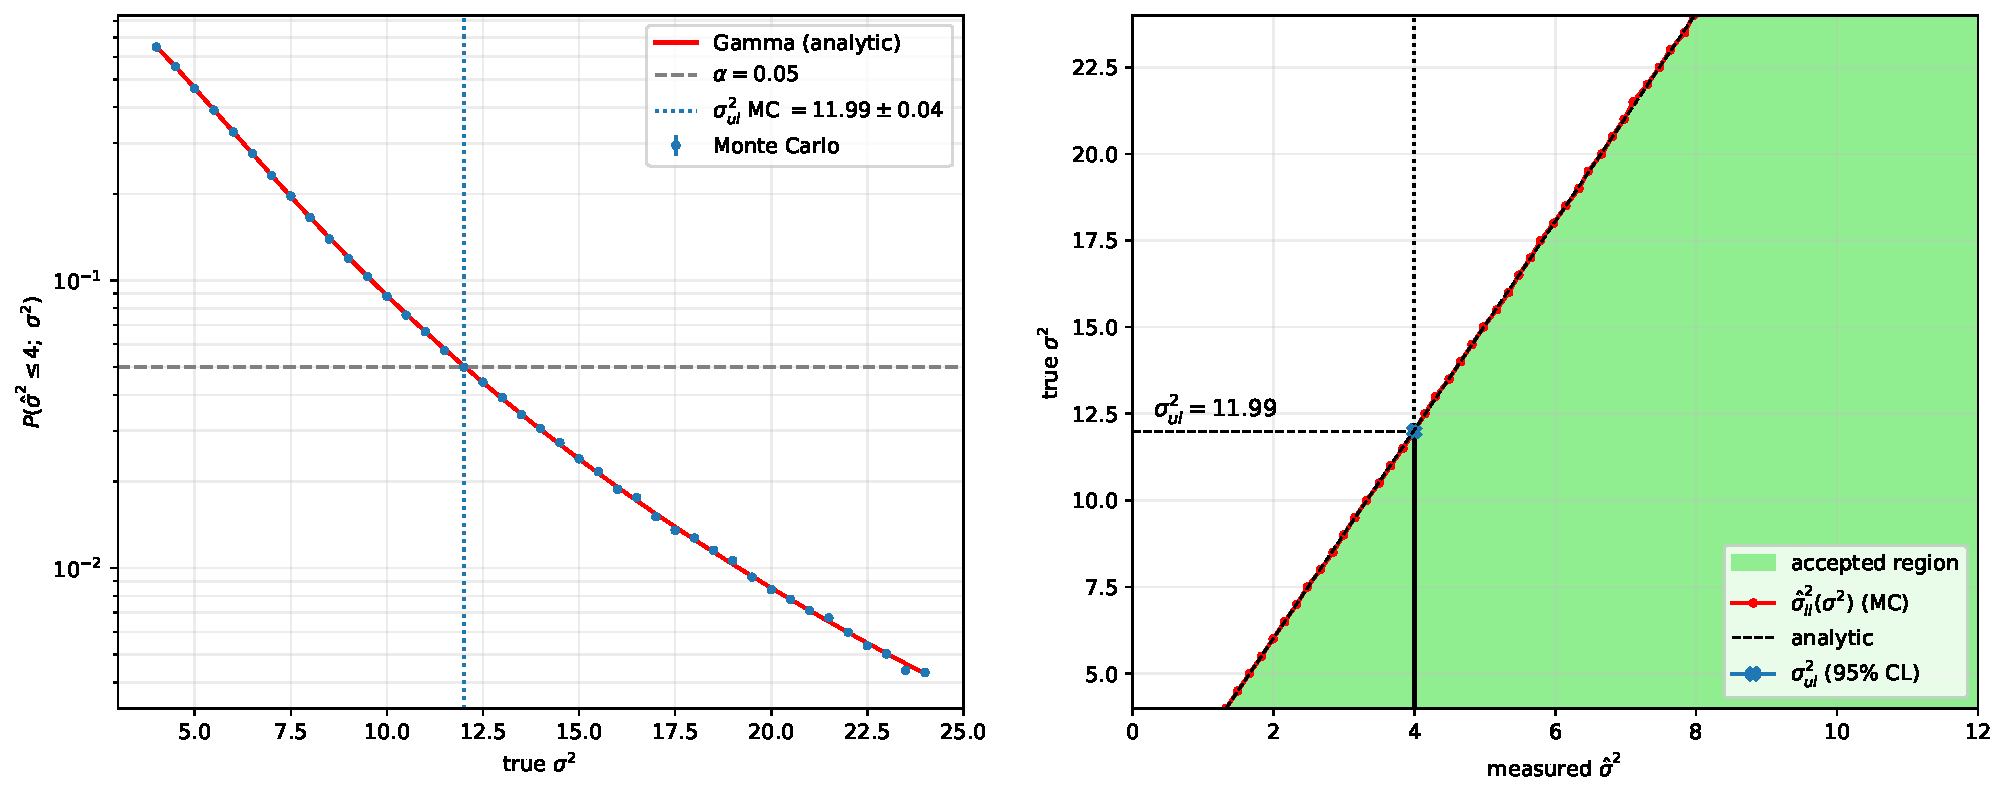
\includegraphics[width=\linewidth]{images/upper_limit_mc.pdf}
		\caption{Left: fraction of simulated experiments with $\hat\sigma^2 \leq 4$ as a function of the true variance, with binomial error bars, compared with the analytic probability. Right: confidence belt obtained from the 5\% quantile of the simulated $\hat\sigma^2$, compared with the analytic boundary $\hat\sigma^2_{ll} = z_\alpha \sigma^2 / N$; the upper limit is where the measurement $\hat\sigma^2_m = 4$ meets the boundary of the accepted region.}
		\label{fig:ul_mc}
	\end{figure}
	\FloatBarrier

	\section*{Conclusions}

	The 95\% CL frequentist upper limit on the variance, obtained from the Gamma distribution of $z = N\hat\sigma^2/\sigma^2$, is
	\begin{equation}
		\sigma^2 < 12.03 \qquad (\sigma < 3.47).
	\end{equation}
	The limit is about three times the measured value $\hat\sigma^2_m = 4$, because $\hat\sigma^2$ has a large and asymmetric spread for only $N = 10$ measurements.
	For a larger number of measurements the distribution of $\hat\sigma^2$ becomes narrower and the upper limit approaches the measured value.

	The Monte Carlo construction, which does not use the Gamma distribution, gives $\sigma^2_{ul} = 11.99 \pm 0.04$, compatible with the analytic result within one standard deviation.
	The estimates from the probability $P(\hat\sigma^2 \leq 4;\ \sigma^2)$ and from the accepted region agree because they are based on the same simulated samples: the $\alpha$-quantile is equal to $\hat\sigma^2_m$ exactly where the fraction of experiments below $\hat\sigma^2_m$ is equal to $\alpha$.
	The residual difference, of order $10^{-4}$, may be due to the linear interpolation between grid points, which is applied to two different curves.


\end{document}
